\chapter{Introduction}

% ====================================================================
\section{Overview}
% ====================================================================

In recent years, digital transformation has expanded to become a truly global phenomenon. Traditional systems in industries such as education, finance, and healthcare are being upgraded with the adoption of artificial intelligence (AI), cloud computing, and blockchain technology \cite{zhang2021}. The term \textit{smart healthcare} refers to the systematic incorporation of electronic means into medical treatment. Using Electronic Health Records (EHRs), mobile internet, wearable technology, and other connected health infrastructure, remote patient monitoring entails collecting, storing, and analysing relevant patient data in real time. The insights gained from continuous monitoring can be used for more accurate illness detection, proactive disease management, and preventive intervention. As a direct consequence, healthcare providers gain the capacity to deliver more personalised, efficient, and timely care to their patients while simultaneously reducing the administrative burden associated with traditional paper-based record systems \cite{tian2019,mohanty2016}.

Despite its many advantages, smart healthcare introduces a set of challenges that remain to be resolved before these systems can reach their full potential. Security and privacy concerns, bandwidth constraints, and latency issues are prominent among these difficulties. Spoofing, cloud polling, radio-frequency (RF) jamming, and Denial-of-Service (DoS) attacks are some of the threats that can befall devices used in smart healthcare networks. Data transmissions frequently traverse networks operated by third parties, increasing exposure to interception and manipulation. These vulnerabilities can endanger both medical facilities and individual patients \cite{zeadally2020}. Electronic health records are particularly susceptible to a wide range of security threats because they contain sensitive personal and clinical information. If such information were to be leaked or tampered with, patients' well-being could be severely jeopardised. A breach of this nature might lead to serious consequences - for example, an attacker posing as a legitimate patient to gain access to medical records or altering prescribed treatments in ways that cause direct physical harm \cite{alomar2021}.

% ====================================================================
\section{Healthcare Insurance}
% ====================================================================

A health insurance policy, commonly abbreviated as HI, is a contractual agreement between an insurance provider and a policyholder whereby the insurer undertakes to cover specified medical costs incurred by the insured party. Losses arising from accidents, hospitalisation, incapacity, unintentional injury, and related damages are among the categories that HI can help compensate for, as broadly defined by the Health Insurance Association of America \cite{healthinsurance2021}. Policyholders are required to make regular premium payments in exchange for this coverage. The insurance entity may be a private commercial company or a government-operated public agency. The persistently rising cost of healthcare services has made health insurance an increasingly essential financial product for modern consumers, with additional incentives provided by the tax advantages that accompany many HI schemes \cite{sheshasaayee2018}. Historically, filing a Health Insurance Claim (HIC) required policyholders to visit an insurance office in person during restricted business hours, complete voluminous forms manually, and then await a response regarding their claim status - a process both inefficient and prone to human error. This reliance on paper-based workflows and manual human resources made HIC audits disproportionately labour-intensive.

The digitalisation of healthcare insurance processes has yielded substantial improvements in efficiency, transparency, and accountability. Maintaining and integrating paper-based health claim records was a complex and time-consuming undertaking that introduced multiple points of failure and opportunities for data manipulation. Digital systems, by contrast, offer the following key advantages:

\begin{enumerate}[label=\roman*.]
    \item \textbf{Reduced processing time:} Claims can be submitted, validated, and adjudicated electronically within hours rather than days or weeks.
    \item \textbf{Lower administrative costs:} Automation of routine processing tasks reduces the need for large clerical workforces, cutting overhead.
    \item \textbf{Improved accuracy:} Automated data validation reduces transcription errors and inconsistencies inherent in manual data entry.
    \item \textbf{Greater transparency:} Digital audit trails allow regulators, providers, and policyholders to trace the full lifecycle of any claim.
    \item \textbf{Enhanced accessibility:} Online portals and mobile applications enable policyholders to submit claims, track status, and access policy information at any time and from any location.
    \item \textbf{Better integration:} Digital platforms facilitate seamless exchange of information among hospitals, diagnostic laboratories, pharmacies, and insurers, reducing duplication and improving care coordination.
\end{enumerate}

Despite these benefits, digitisation has also introduced new attack surfaces for fraudulent actors who exploit the scale, speed, and complexity of digital claims processing systems to perpetrate healthcare fraud with greater sophistication than was previously possible \cite{patil2014}.

% ====================================================================
\section{Healthcare Fraud}
% ====================================================================

In the healthcare sector, the term \textit{healthcare fraud} refers to any instance of intentional, unlawful deceit or misrepresentation of information carried out with the intent to obtain an illicit financial advantage. It encompasses a broad range of illegal actions undertaken to improperly receive healthcare funds, goods, or services from government healthcare programs, private health insurers, or individual patients. The negative consequences of healthcare fraud are wide-ranging and include higher overall healthcare expenditures for all participants in the system, diminished quality of treatment for genuine patients, and significant financial losses for both healthcare providers and publicly funded healthcare programs \cite{macfarlane2020}.

There are many distinct categories of HI fraud, and several different parties are typically involved in any given fraud scheme. Broadly, three principal actors are implicated. First, healthcare service providers - comprising physicians, hospitals, ambulance services, and diagnostic centres - who may misrepresent or fabricate the services rendered. Second, HI subscribers such as individual patients and their employers, who may provide false information at the point of enrolment or at the time of making a claim. Third, HI providers themselves - including private insurance companies and public health agencies - who may engage in unfair denial of legitimate claims, policy misrepresentation, or premium manipulation \cite{duman2017}. Figure~\ref{fig:fraud_types} presents a taxonomic overview of the principal categories of health insurance fraud.

% -------------------------------------------------------
% Figure 1.2 -- Types of Health Insurance Frauds (TikZ)
% -------------------------------------------------------
\begin{figure}[H]
\centering
% TikZ tree diagram: Types of Health Insurance Fraud
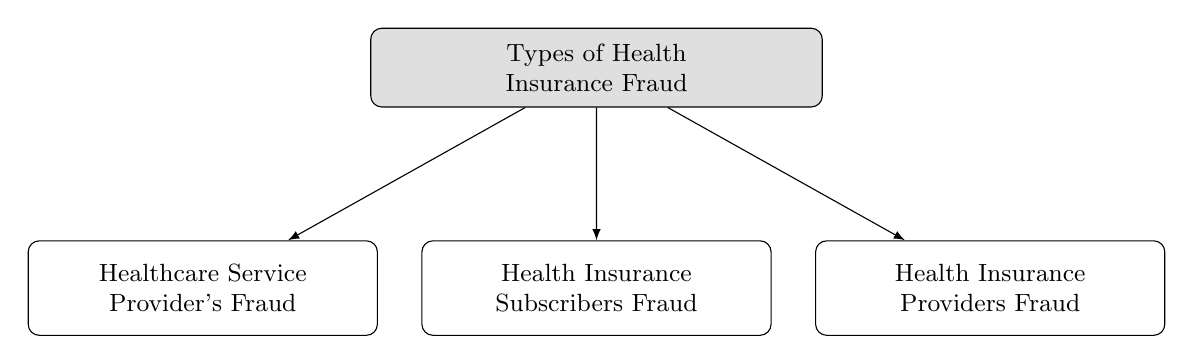
\begin{tikzpicture}[
    every node/.style={draw, rounded corners, align=center, font=\small},
    root/.style={fill=gray!25, text width=5.5cm, minimum height=1cm},
    child/.style={fill=white, text width=4.2cm, minimum height=1.2cm},
    level 1/.style={sibling distance=5cm, level distance=2.8cm},
    edge from parent/.style={draw, -latex}
]
\node[root] {Types of Health\\Insurance Fraud}
    child { node[child] {Healthcare Service\\Provider's Fraud} }
    child { node[child] {Health Insurance\\Subscribers Fraud} }
    child { node[child] {Health Insurance\\Providers Fraud} };
\end{tikzpicture}
\caption{Types of Health Insurance Fraud}
\label{fig:fraud_types}
\end{figure}

% -------------------------------------------------------
\subsection{Healthcare Service Provider's Fraud}
% -------------------------------------------------------

Healthcare service provider fraud involves deliberate misrepresentation or fabrication of clinical activities by those responsible for delivering medical care. Common manifestations include billing for services that were never rendered, upcoding - whereby a provider submits a claim for a more expensive service or procedure than was actually performed, unbundling - the practice of billing separately for component procedures that should be billed together at a lower aggregate cost, and duplicate billing for the same service across multiple claims submissions \cite{kose2015}. Providers may also engage in phantom billing, where services are invoiced on behalf of patients who do not exist or who were not present. More elaborate schemes involve kickback arrangements in which providers accept or pay referral fees in exchange for steering patients toward particular tests, treatments, or facilities regardless of clinical need. The financial incentives embedded in fee-for-service reimbursement structures create a systemic vulnerability that sophisticated fraudsters exploit through careful manipulation of billing codes and clinical documentation, making such fraud difficult to identify through manual auditing alone \cite{rayan2019}.

% -------------------------------------------------------
\subsection{HI Subscribers Fraud}
% -------------------------------------------------------

Health insurance subscriber fraud is perpetrated by policyholders - either individual patients or their employers - who deliberately misrepresent information in order to obtain coverage or reimbursement to which they are not entitled. Common subscriber-level fraud schemes include providing false personal or medical history information during the enrolment process in order to secure a lower premium, submitting claims for medical services that were never received, misrepresenting the identity of the insured person by allowing a non-covered individual to use an active policy holder's insurance credentials, and inflating the cost of legitimate medical expenses beyond what was actually incurred \cite{ahmed2014}. Subscribers may also collude with service providers to create fictitious claims, a form of cooperative fraud that is particularly difficult to detect because it involves documentation that is consistent across multiple independent data sources. The growing availability of stolen personal identity data on underground digital markets has further amplified subscriber-level fraud, as stolen credentials are used to generate fraudulent insurance claims at scale without the knowledge of the legitimate policy holder \cite{thaifur2021}.

% -------------------------------------------------------
\subsection{HI Providers Fraud}
% -------------------------------------------------------

Fraud perpetrated by health insurance providers - the insurance companies and agencies themselves - represents a less commonly discussed but equally damaging category of healthcare fraud. This form of fraud typically operates to the detriment of policyholders and the broader regulatory ecosystem. Specific practices include deliberate misrepresentation of policy terms and coverage at the point of sale, unjustified denial of legitimate claims through manipulation of pre-existing condition clauses or policy exclusions, improper delay in claims adjudication to benefit from the time-value of premium income, and the sale of fraudulent or non-existent insurance products by unlicensed entities to unsuspecting consumers \cite{zhu2021}. Insurance providers operating in less regulated markets may also engage in data manipulation - falsifying actuarial reports, misreporting claims ratios to regulators, or under-reserving for known liabilities. As health insurance markets have grown increasingly complex, regulatory oversight has struggled to keep pace with the sophistication of provider-level fraud schemes, particularly in markets with fragmented oversight across multiple state or provincial jurisdictions \cite{sun2018patient}.

% ====================================================================
\section{Fraud Prevention in Health Insurance}
% ====================================================================

Healthcare fraud is estimated to cost the global healthcare system between \$125 billion and \$175 billion annually, representing a substantial proportion of total healthcare expenditure that is diverted away from genuine patient care \cite{healthinsurance2021,macfarlane2020}. In the United States alone, the National Health Care Anti-Fraud Association estimates that the financial burden of healthcare fraud amounts to approximately 3 to 10 percent of total health spending each year. Beyond the direct financial losses, fraud drives up insurance premiums for honest policyholders, degrades the quality of care available to patients, erodes trust in healthcare institutions, and diverts resources that could otherwise fund legitimate medical research and infrastructure. The problem is compounded by the fact that only a small fraction of fraudulent claims are ever detected, investigated, and prosecuted - largely because traditional detection mechanisms are inadequate in the face of the volume, velocity, and variety of claims data generated by modern healthcare systems \cite{zhou2020}.

Traditional fraud detection methods rely primarily on manual auditing, retrospective claims review, and rule-based expert systems that encode domain knowledge into fixed sets of pre-defined detection criteria. While these approaches provide a useful baseline, they suffer from fundamental limitations. Rule-based systems require constant manual maintenance as fraud patterns evolve, are unable to detect novel fraud schemes that deviate from known patterns, generate high false-positive rates that impose significant investigative costs, and cannot efficiently scale to process the billions of claims submitted each year across global healthcare systems \cite{tsai2019}. The emergence of machine learning (ML) techniques and distributed ledger technologies such as blockchain presents a promising opportunity to address these limitations. ML classifiers can identify complex, non-linear statistical relationships between claims features that are indicative of fraud, even when individual features appear unremarkable in isolation. Blockchain provides an immutable, cryptographically secured audit trail for the claims adjudication process, ensuring that detection results and the underlying data upon which they are based remain tamper-evident and auditable by all authorised parties \cite{hilal2022}.

% ====================================================================
\section{Machine Learning and Blockchain for Healthcare Fraud Prevention}
% ====================================================================

Machine learning approaches to healthcare fraud detection operate by learning statistical patterns that distinguish fraudulent from legitimate claims using historical labelled data. Supervised learning algorithms - including gradient-boosted decision trees, random forests, neural networks, and logistic regression - have demonstrated strong performance on fraud detection benchmarks by exploiting the rich feature space available in structured claims data \cite{wang2021deep}. Features derived from billing codes, provider speciality, patient demographics, claim frequency, temporal patterns, and reimbursement amounts collectively provide a high-dimensional representation of each claim that ML models can use to assign a fraud probability score. Ensemble methods that combine the predictions of multiple base learners are particularly effective because they reduce variance, mitigate overfitting, and capture complementary aspects of the fraud signal that no single model can detect in isolation \cite{tenepalli2022}. Advanced interpretability tools such as SHAP (SHapley Additive exPlanations) and LIME (Local Interpretable Model-agnostic Explanations) enable auditors to understand why any given claim was flagged, satisfying the transparency requirements of regulatory frameworks such as HIPAA and the EU General Data Protection Regulation \cite{li2021}.

Blockchain technology complements ML-based detection by providing an immutable, decentralised ledger on which fraud prediction results, feature vectors, and claims metadata can be recorded with cryptographic integrity guarantees. Once a record is appended to the blockchain, it cannot be modified or deleted without invalidating the entire subsequent chain, providing a tamper-evident audit trail that is resistant to post-hoc manipulation by any single party. Smart contracts can encode the business logic of claims adjudication, automatically triggering investigative workflows when an ML model assigns a fraud score exceeding a defined threshold \cite{alhashedi2021}. The combination of Elliptic Curve Integrated Encryption Scheme (ECIES) for encrypting sensitive patient data and SHA-256 hashing for block integrity ensures that the privacy of individual patients is preserved while the overall transparency and auditability of the fraud detection process is maintained for authorised reviewers \cite{amponsah2022}. Figure~\ref{fig:ml_blockchain_arch} illustrates the high-level architecture of the proposed ML and blockchain integrated fraud detection pipeline.

% -------------------------------------------------------
% Figure 1.2 -- ML + Blockchain Architecture (snake/zigzag layout)
% -------------------------------------------------------
\begin{figure}[H]
\centering
\begin{tikzpicture}[
    node distance=0.9cm and 0.6cm,
    data/.style={draw, rounded corners=3pt, fill=green!12, minimum width=4.6cm,
                 minimum height=0.75cm, align=center, font=\small\bfseries, thick},
    proc/.style={draw, rounded corners=3pt, fill=blue!10, minimum width=4.6cm,
                 minimum height=0.75cm, align=center, font=\small, thick},
    ml/.style={draw, rounded corners=3pt, fill=orange!12, minimum width=4.6cm,
               minimum height=0.75cm, align=center, font=\small, thick},
    sec/.style={draw, rounded corners=3pt, fill=red!8, minimum width=4.6cm,
                minimum height=0.75cm, align=center, font=\small, thick},
    outp/.style={draw, rounded corners=3pt, fill=yellow!15, minimum width=4.6cm,
                minimum height=0.75cm, align=center, font=\small, thick},
    arrow/.style={-latex, thick, color=gray!70},
    layer/.style={font=\scriptsize\itshape, text=gray}
]
% Row 1 (left to right): Data Layer
\node[layer] at (-3.8, 0.6) {Data Layer};
\node[data] (raw) at (0, 0) {CMS Medicare Claims};
\node[data, right=of raw] (merge) {Merge 4 CSVs (558K rows)};

% Row 2 (right to left): Feature Layer
\node[layer] at (-3.8, -1.4) {Feature Layer};
\node[proc, below=of merge] (agg) {Provider Aggregation (5,410)};
\node[proc, left=of agg] (feat) {190 Feature Engineering};

% Row 3 (left to right): ML Layer
\node[layer] at (-3.8, -3.4) {ML Layer};
\node[ml, below=of feat] (optuna) {Optuna HPO (60 trials)};
\node[ml, right=of optuna] (train) {10-Fold Stratified CV};

% Row 4 (right to left): Decision Layer
\node[layer] at (-3.8, -5.4) {Decision Layer};
\node[ml, below=of train] (pred) {XGBoost Prediction};
\node[outp, left=of pred] (thresh) {Fixed Threshold $t{=}0.5$};

% Row 5 (left to right): Security + Explainability Layer
\node[layer] at (-3.8, -7.4) {Security Layer};
\node[sec, below=of thresh] (ecies) {ECIES Encryption};
\node[sec, right=of ecies] (chain) {SHA-256 Blockchain};

% Row 6 (right to left): Output Layer
\node[layer] at (-3.8, -9.4) {Output Layer};
\node[outp, below=of chain] (shap) {SHAP Explainability};
\node[outp, left=of shap] (lime) {LIME Case Studies};

% Arrows: snake pattern
\draw[arrow] (raw) -- (merge);
\draw[arrow] (merge) -- (agg);
\draw[arrow] (agg) -- (feat);
\draw[arrow] (feat) -- (optuna);
\draw[arrow] (optuna) -- (train);
\draw[arrow] (train) -- (pred);
\draw[arrow] (pred) -- (thresh);
\draw[arrow] (thresh) -- (ecies);
\draw[arrow] (ecies) -- (chain);
\draw[arrow] (chain) -- (shap);
\draw[arrow] (shap) -- (lime);

% Feedback arrow from SHAP back to threshold
\draw[arrow, dashed, color=blue!50] (lime.south) -- ++(0,-0.4) -| ([xshift=-0.5cm]thresh.south) node[midway, below, font=\scriptsize, text=blue!60] {Audit Feedback};

\end{tikzpicture}
\caption{High-level architecture of the proposed ML and blockchain-based healthcare fraud detection pipeline. The snake layout illustrates the sequential data flow through six functional layers: data ingestion, feature engineering, model training, decision making, cryptographic security, and explainability output.}
\label{fig:ml_blockchain_arch}
\end{figure}

% ====================================================================
\section{Innovative Healthcare Insurance Fraud Detection}
% ====================================================================

The field of healthcare insurance fraud detection has undergone a significant methodological evolution over the past two decades, progressing from simple rule-based filters and manual audit sampling toward sophisticated data-driven systems that employ statistical learning, graph analysis, and distributed ledger technologies. Early detection systems were characterised by their reliance on fixed heuristics derived from known fraud patterns, which made them straightforwardly circumventable by fraudsters who adapted their schemes to avoid triggering pre-defined rules. The emergence of large-scale administrative claims databases - particularly the publicly available Centers for Medicare and Medicaid Services (CMS) datasets - has enabled the development and rigorous empirical evaluation of ML-based detection approaches at a scale and with a degree of reproducibility that was previously impossible \cite{ahmadian2020}. Modern approaches increasingly combine multiple complementary detection modalities, integrating supervised classification for provider-level fraud scoring, unsupervised anomaly detection for identifying novel fraud typologies, network analysis for uncovering collusion among providers, and blockchain-based audit trails for ensuring the integrity and non-repudiation of detection outcomes \cite{hassan2019}.

The present research contributes to this body of work by proposing and empirically validating a rigorous, reproducible pipeline for provider-level fraud detection that emphasises proper evaluation methodology, stratified cross-validation, and a systematic investigation of whether synthetic oversampling genuinely improves performance on imbalanced healthcare fraud datasets. The specific research objectives motivating this work are as follows:

\begin{enumerate}[label=\roman*.]
    \item To design and implement a rigorous feature engineering and normalisation pipeline for the CMS Medicare Part B provider-level fraud detection dataset, ensuring that all preprocessing steps respect the train-test boundary.
    \item To apply Bayesian hyperparameter optimisation using Optuna across five candidate machine learning classifiers - XGBoost, LightGBM, Gradient Boosting, CatBoost, and Random Forest - with stratified cross-validation to identify the best-performing configuration.
    \item To conduct a systematic ablation study on the effect of SMOTE-ENN synthetic oversampling on model performance under proper evaluation conditions, and to challenge the prevailing assumption that oversampling is universally beneficial for imbalanced fraud datasets.
    \item To integrate a SHA-256 blockchain with ECIES-encrypted patient data and smart contract-triggered investigative workflows into the fraud detection pipeline, thereby ensuring tamper-evidence, auditability, and privacy compliance.
    \item To provide comprehensive post-hoc model explainability through SHAP and LIME analyses, enabling human auditors to understand, validate, and trust the individual fraud classification decisions produced by the model.
\end{enumerate}

% ====================================================================
\section{Fraud Detection Issues and Challenges}
% ====================================================================

Healthcare fraud detection is a technically demanding problem that sits at the intersection of data science, information security, regulatory compliance, and clinical domain expertise. While machine learning and blockchain technologies offer powerful new tools for addressing fraud, their effective deployment in real-world healthcare systems requires navigating a complex landscape of interrelated challenges. This section provides a structured overview of the principal issues that practitioners must contend with when designing and deploying fraud detection systems for health insurance applications \cite{cruz2017,liang2019}.

% -------------------------------------------------------
\subsection{Sophisticated Fraud Schemes}
% -------------------------------------------------------

Modern healthcare fraud perpetrators employ increasingly sophisticated techniques designed specifically to evade detection by both human auditors and automated systems. Organised fraud networks coordinate the activities of multiple providers, clinics, and patient recruiters to generate large volumes of claims that are individually plausible but collectively fraudulent \cite{choi2020}. Collusive fraud schemes are particularly challenging because the consistency of documentation across multiple independent data sources makes them appear legitimate under standard single-entity audit procedures. As detection algorithms improve and are deployed at scale, fraudsters adapt their methods through a process akin to adversarial learning - subtly modifying billing patterns, rotating provider identities, and introducing noise to remain below algorithmic detection thresholds. This adversarial dynamic necessitates continuous model retraining and evaluation against evolving fraud distributions rather than treating detection as a one-time model deployment exercise.

% -------------------------------------------------------
\subsection{Data Volume and Variety}
% -------------------------------------------------------

National healthcare systems process hundreds of millions of insurance claims annually, generating datasets of substantial size and complexity. The CMS Medicare system alone adjudicates over one billion claims per year across Part A (inpatient), Part B (outpatient and physician), and Part D (prescription drug) programs. Effective fraud detection at this scale requires systems capable of processing high-velocity data streams in near real time, often within the latency constraints of automated adjudication workflows \cite{kumar2020}. Beyond sheer volume, healthcare claims data exhibits significant structural variety - incorporating diagnostic codes from the International Classification of Diseases (ICD), procedure codes from the Current Procedural Terminology (CPT), revenue codes, provider taxonomy codes, National Drug Codes (NDC), and demographic information - each governed by its own coding standards, versioning histories, and domain-specific semantics that must be correctly interpreted to extract meaningful fraud signals.

% -------------------------------------------------------
\subsection{Data Quality}
% -------------------------------------------------------

The effectiveness of any data-driven fraud detection system is fundamentally bounded by the quality of the underlying data. Healthcare administrative data is subject to a range of quality issues including missing values arising from optional fields in claim submission standards, systematic coding errors introduced by medical billing software, inconsistent use of modifier codes across providers and regions, and duplicate claim submissions arising from billing system errors rather than intentional fraud \cite{singh2021}. The presence of these data quality issues means that a significant pre-processing investment is required before any ML model can be reliably trained. Imputation strategies for missing values must be carefully chosen to avoid introducing bias into the feature space; for example, mean imputation for skewed reimbursement amounts can systematically underestimate the true degree of provider billing variability that is itself a fraud signal. The pipeline described in this work devotes substantial attention to reproducible pre-processing as a foundational requirement for valid model evaluation.

% -------------------------------------------------------
\subsection{Connecting to Outdated Computer Systems}
% -------------------------------------------------------

A significant practical barrier to the deployment of advanced fraud detection systems in healthcare is the prevalence of legacy information technology infrastructure across hospitals, insurers, and government health agencies. Many organisations continue to operate claims processing systems built on decades-old mainframe architectures or early-generation relational database management systems that predate modern data science tooling \cite{buczak2016}. Integrating ML-based detection modules with these legacy systems requires the development of bespoke data extraction, transformation, and loading (ETL) pipelines that can bridge incompatible data formats, authentication protocols, and network architectures. In many cases, real-time data feeds are not technically feasible, limiting fraud detection to retrospective batch analysis that introduces a lag between the time a fraudulent claim is submitted and the time it is flagged - during which additional fraudulent claims from the same actor may be processed and paid.

% -------------------------------------------------------
\subsection{Privacy Concerns}
% -------------------------------------------------------

Healthcare data is among the most sensitive categories of personal information, subject to strict regulatory protection under frameworks including the Health Insurance Portability and Accountability Act (HIPAA) in the United States, the General Data Protection Regulation (GDPR) in the European Union, and equivalent national legislation in jurisdictions worldwide \cite{he2019}. Fraud detection systems necessarily require access to detailed claims data that contains or can be linked to individually identifiable patient information. Balancing the need for analytical access to support fraud detection against the legal and ethical obligations to protect patient privacy requires careful system design. Techniques such as data anonymisation, differential privacy, federated learning, and field-level encryption - as employed through ECIES in this work - provide partial solutions, but each introduces trade-offs in detection accuracy, computational cost, or operational complexity that must be explicitly managed.

% -------------------------------------------------------
\subsection{Lack of Standardization}
% -------------------------------------------------------

Healthcare data standards vary considerably across countries, health systems, insurance products, and time periods. Diagnostic coding systems have transitioned from ICD-9 to ICD-10 and are moving toward ICD-11, while procedure coding varies between CPT, HCPCS, and national equivalents. These transitions create temporal discontinuities in claims databases that can mislead models trained on historical data when applied to current claims \cite{eling2018}. Beyond coding standards, the lack of a universal provider identifier, inconsistent definitions of claim fields across payer systems, and heterogeneous data exchange formats all impede the development of fraud detection models that can be readily generalised from one health system or insurance market to another. This fragmentation of standards also complicates the creation of cross-institutional datasets large enough to support robust training of deep learning models.

% -------------------------------------------------------
\subsection{Security of HI System}
% -------------------------------------------------------

The healthcare insurance system is not only vulnerable to fraud from external actors but also faces internal security threats from employees who have privileged access to claims data and adjudication systems \cite{elemam2013}. Insider threats may involve the deliberate manipulation of claims outcomes, the disclosure of patient data to external fraud networks, or the sabotage of fraud detection workflows. Beyond insider threats, healthcare information systems are high-value targets for external cyberattacks including ransomware campaigns that encrypt claims databases and demand payment for their restoration. A robust fraud detection infrastructure must therefore incorporate information security controls - including role-based access control, multi-factor authentication, encrypted data-at-rest and data-in-transit, and continuous security monitoring - that protect both the integrity of fraud detection outcomes and the confidentiality of the patient data on which they are based.

% -------------------------------------------------------
\subsection{Resource Constraints}
% -------------------------------------------------------

Effective fraud detection requires sustained investment in computational infrastructure, data science expertise, and operational processes for investigating and acting on flagged claims \cite{yoo2015}. Many health insurance organisations - particularly smaller regional insurers and government health programs in lower-income countries - lack the financial and human capital resources to develop and maintain sophisticated ML-based detection systems. Open-source tools and cloud-based computing services have substantially reduced the barrier to entry for deploying ML models, but the operational costs of model maintenance, re-training, and continuous evaluation remain non-trivial. The Special Investigation Unit (SIU) investigators who must follow up on algorithmically flagged claims represent a fixed investigative capacity that can easily be overwhelmed if detection systems generate large volumes of false positives, creating a practical ceiling on the effective sensitivity of deployed fraud detection systems.

% -------------------------------------------------------
\subsection{Cross-Channel Fraud}
% -------------------------------------------------------

Modern healthcare fraud increasingly operates across multiple channels and claim types simultaneously, exploiting inconsistencies between the oversight mechanisms applied to different segments of the healthcare system \cite{kumar2011}. A single fraud scheme may involve fabricated inpatient claims submitted under Part A, inflated physician billing under Part B, and fraudulent prescription drug claims under Part D - with each component appearing normal when examined in isolation within its own program but revealing a coordinated pattern only when data across programs is integrated and analysed jointly. Cross-channel fraud detection therefore requires not only within-channel anomaly detection but also the capacity to link identities and activities across disparate data sources, which is technically challenging when provider and patient identifiers are not consistently maintained across systems.

% -------------------------------------------------------
\subsection{Regulatory Challenges}
% -------------------------------------------------------

Healthcare fraud detection systems operate within a complex and evolving regulatory environment that constrains both the data that may be used for detection and the actions that may be taken in response to flagged claims \cite{dutt2020}. Regulations governing data retention, patient consent, algorithmic decision-making, and anti-discrimination must all be observed when designing and deploying automated detection systems. Increasingly, regulatory frameworks are demanding explainability for automated decisions that affect individuals - including the denial or investigation of insurance claims - which places additional requirements on the interpretability of detection models beyond what would be required purely on accuracy grounds. In the European Union, the AI Act introduces specific obligations for AI systems used in high-risk contexts such as healthcare, requiring conformity assessments, transparency disclosures, and human oversight provisions that must be built into the detection pipeline from the outset.

% -------------------------------------------------------
\subsection{Machine Learning and AI Limitations}
% -------------------------------------------------------

While ML techniques have demonstrated strong empirical performance on historical fraud detection benchmarks, they carry inherent limitations that are particularly consequential in the healthcare domain \cite{gerke2019}. Class imbalance is a fundamental challenge: in most healthcare claims datasets, fraudulent claims constitute a small minority of total records, creating a statistical environment in which a classifier that labels all claims as legitimate can achieve deceptively high accuracy. Standard performance metrics such as overall accuracy therefore fail to capture the practically relevant capability of the model to correctly identify the fraudulent minority. The pipeline in this work uses AUC-PR (Area Under the Precision-Recall Curve) as the primary optimisation objective, a choice that directly addresses this imbalance by emphasising performance on the positive (fraud) class. ML models are also susceptible to distribution shift - their performance degrades when the statistical characteristics of current claims data diverge from those of the training set - necessitating regular re-evaluation and re-training against updated data.

% -------------------------------------------------------
\subsection{Human Expertise}
% -------------------------------------------------------

Despite the potential of automated systems to process data at a scale and speed beyond human capacity, healthcare fraud detection ultimately requires deep collaboration between algorithmic systems and experienced human investigators \cite{abdallah2016}. Clinical domain expertise is indispensable for interpreting the significance of specific billing patterns, understanding the legitimate clinical rationale for unusual treatment sequences, and exercising judgment in ambiguous cases where algorithmic scores alone are insufficient to determine fraud. Experienced investigators also play a critical role in providing labelled data through confirmed fraud cases, feeding the supervised learning pipeline that underpins model training. The scarcity of this expertise - combined with high investigator turnover, institutional knowledge loss, and the cognitive burden of reviewing large volumes of algorithmically flagged cases - represents a persistent bottleneck in the operationalisation of fraud detection systems, regardless of their algorithmic sophistication.

% ====================================================================
\section{Taxonomy of Health Insurance Fraud Detection}
% ====================================================================

The academic and applied literature on health insurance fraud detection encompasses a rich diversity of methodological approaches, each with distinct strengths, limitations, and areas of applicability. Structuring this diversity into a coherent taxonomy facilitates comparative evaluation and helps practitioners select the most appropriate detection strategy for a given operational context. The principal methodological families are reviewed in the following subsections, drawing on a representative selection of landmark studies to illustrate the capabilities and limitations of each approach \cite{pareek2023,hilal2022}.

% -------------------------------------------------------
\subsection{Supervised Learning}
% -------------------------------------------------------

Supervised learning approaches train classification models using labelled historical data in which individual claims or providers have been identified as either fraudulent or legitimate by human investigators or regulatory authorities \cite{duman2017}. A wide range of supervised algorithms has been applied to HI fraud detection, including logistic regression, decision trees, random forests, gradient-boosted machines, support vector machines, and deep neural networks. The primary strength of supervised approaches is their capacity to learn highly non-linear discriminative boundaries in high-dimensional feature spaces, enabling them to detect complex fraud patterns that would be invisible to rule-based systems. The principal limitation is their dependence on large quantities of accurately labelled training data, which is expensive and time-consuming to produce and is frequently subject to label noise arising from cases where fraud was suspected but not definitively proven. Class imbalance is an additional structural challenge, as fraudulent claims typically represent a small fraction of total claims volume, and standard training objectives can cause models to over-fit to the majority class at the expense of fraud detection sensitivity \cite{kose2015}.

% -------------------------------------------------------
\subsection{Unsupervised Learning}
% -------------------------------------------------------

Unsupervised learning methods detect fraud by identifying claims or providers whose statistical characteristics deviate significantly from the norm without requiring prior labelled examples of fraud \cite{zhou2020}. Clustering algorithms such as k-means, DBSCAN, and Gaussian mixture models partition the claims population into groups of similar entities and flag members of small or outlying clusters as anomalous. Autoencoders and other deep generative models learn a compact latent representation of normal claims data and detect fraud through elevated reconstruction error on claims that do not conform to learned normal patterns. The principal advantage of unsupervised approaches is their ability to detect novel fraud typologies that have not been previously observed and thus cannot be captured by supervised models trained on historical fraud labels. Their limitation is the absence of a direct optimisation objective tied to fraud detection, which can result in high false-positive rates as legitimate but unusual claims are flagged alongside genuinely fraudulent ones \cite{tsai2019}.

% -------------------------------------------------------
\subsection{Hybrid Approach}
% -------------------------------------------------------

Hybrid approaches combine supervised and unsupervised techniques to capitalise on the complementary strengths of each paradigm. A common architecture uses an unsupervised anomaly detector as a first-stage filter to identify suspicious claims warranting closer examination, followed by a supervised classifier trained on confirmed fraud labels to make a final determination on the pre-filtered set \cite{wang2021deep}. Alternatively, unsupervised clustering can be used to generate pseudo-labels for unlabelled data, which are then used to augment a supervised training set in a semi-supervised learning framework. Hybrid approaches have demonstrated improvements in both precision and recall relative to either pure supervised or pure unsupervised baselines in multiple published evaluations, and they offer a practical pathway for deploying effective fraud detection in settings where labelled data is scarce \cite{ahmadian2020}. The ensemble architecture adopted in this work - combining Optuna-tuned XGBoost, LightGBM, CatBoost, and other classifiers through a voting scheme - represents a form of supervised ensemble hybridisation that benefits from diversity among base learners.

% -------------------------------------------------------
\subsection{HIC Fraud Detection from Group of People}
% -------------------------------------------------------

Group-level fraud detection recognises that healthcare fraud is frequently a collective rather than an individual phenomenon, involving coordinated activity among networks of providers, patients, and administrative staff \cite{sun2018patient}. Graph-theoretic and social network analysis methods model the relationships among healthcare entities as a network, with nodes representing providers or patients and edges representing referral relationships, shared billing patterns, or co-occurring diagnoses. Community detection algorithms identify dense subgraphs that may represent collusive fraud rings, while anomalous edge weights or unusual community membership patterns serve as fraud indicators. This approach is particularly effective for detecting the organised fraud schemes that account for a disproportionate share of total fraud losses, as the network structure of these schemes leaves a distinctive statistical signature even when individual transactions appear legitimate in isolation \cite{hassan2019}.

% -------------------------------------------------------
\subsection{Blockchain-Based HIC Fraud Prevention}
% -------------------------------------------------------

Blockchain technology provides a fundamentally different approach to fraud prevention - one focused on making fraud more difficult to perpetrate rather than on detecting it after the fact. By recording claims data, adjudication decisions, and payment transactions on a distributed, immutable ledger, blockchain creates a transparent and tamper-evident audit trail that exposes the data manipulation and identity falsification on which many fraud schemes depend \cite{alhashedi2021}. Smart contracts can enforce claims adjudication rules automatically and consistently, eliminating the discretionary decision-making that is sometimes exploited in manual approval workflows. The cryptographic properties of blockchain - including digital signatures for provider identity verification and hash-based integrity checking for claims data - provide strong authenticity guarantees that are technically very difficult to circumvent. Practical implementations must address challenges of scalability, latency, and interoperability with existing healthcare IT infrastructure, but proof-of-concept systems have demonstrated the viability of blockchain-based fraud prevention in pilot deployments \cite{amponsah2022}.

% -------------------------------------------------------
\subsection{AI and Blockchain-Based HIC Fraud Detection}
% -------------------------------------------------------

The integration of AI and blockchain technologies represents the most comprehensive approach to HI fraud detection currently available, combining the predictive power of machine learning with the auditability and integrity guarantees of distributed ledger technology \cite{li2021}. In such integrated architectures, ML models process claims data in real time to generate fraud probability scores, which are then recorded on the blockchain alongside the encrypted features used to produce them. This creates a verifiable, non-repudiable record of every fraud assessment decision that can be audited by regulators, insurers, and - where appropriate under data protection law - patients themselves. Smart contracts can automate the downstream workflow triggered by high fraud scores, initiating investigative queues, placing payment holds, or notifying relevant oversight authorities without requiring manual intervention \cite{pareek2023}. The SHAP-based explainability layer included in the present work addresses the additional requirement that AI-generated fraud assessments be interpretable by human reviewers, bridging the gap between algorithmic sophistication and operational accountability.

% ====================================================================
\section{Security and Privacy Requirements of Healthcare Applications}
% ====================================================================

Healthcare applications that process, store, or transmit patient and claims data must satisfy a comprehensive set of security and privacy requirements derived from both regulatory mandates and fundamental information security principles. Failure to meet any of these requirements creates vulnerabilities that can be exploited both by fraudsters seeking to manipulate the claims process and by malicious actors seeking to obtain sensitive patient data for identity theft, blackmail, or other harmful purposes. The following subsections describe the principal security and privacy requirements applicable to health insurance fraud detection systems, with reference to their specific relevance in the context of the proposed ML and blockchain-based pipeline \cite{zeadally2020,alomar2021}.

% -------------------------------------------------------
\subsection{Data Confidentiality}
% -------------------------------------------------------

Data confidentiality ensures that sensitive healthcare information is accessible only to those parties with an explicit, authorised need to access it - and is shielded from all other parties including potential eavesdroppers on communication networks and unauthorised internal users \cite{elemam2013}. In the context of health insurance fraud detection, confidentiality applies to patient demographics, diagnosis and procedure codes, provider identities, and reimbursement amounts - all of which are sensitive either individually or in combination. The Elliptic Curve Integrated Encryption Scheme (ECIES) employed in the blockchain component of this work provides strong asymmetric encryption of patient-identifiable data fields before they are committed to the ledger, ensuring that only authorised investigators holding the corresponding private key can decrypt and view individual patient records while the fraud assessment scores remain transparent to auditors.

% -------------------------------------------------------
\subsection{Data Authentication}
% -------------------------------------------------------

Data authentication mechanisms ensure that the provenance of healthcare records can be verified - that a claim, diagnosis code, or treatment record was genuinely submitted by the party that purports to have submitted it, and that it has not been modified in transit or at rest \cite{hassan2019}. In the blockchain component of the proposed system, each block is identified by a SHA-256 cryptographic hash that incorporates the hash of the preceding block, creating a chain structure in which any modification to a historical record immediately invalidates all subsequent hashes and is thus instantly detectable. Digital signatures applied at the point of claim submission further ensure that records can be traced to their originating provider entity, providing non-repudiation guarantees that are essential for supporting legal proceedings against identified fraudsters.

% -------------------------------------------------------
\subsection{Strong User Authentication}
% -------------------------------------------------------

Access to fraud detection systems and the sensitive data they process must be protected by robust user authentication mechanisms that prevent unauthorised individuals from querying fraud scores, accessing patient records, or manipulating detection parameters \cite{yoo2015}. Multi-factor authentication, combining something the user knows (a password), something the user has (a hardware token or mobile device), and optionally something the user is (a biometric factor), provides substantially stronger access control than single-factor password-based authentication, which is vulnerable to credential theft and brute-force attacks. Role-based access control ensures that different categories of system users - data scientists, claims investigators, compliance officers, and patients - have access only to the specific system functions and data fields relevant to their role, implementing the principle of least privilege as a foundational security control.

% -------------------------------------------------------
\subsection{Data Integrity}
% -------------------------------------------------------

Data integrity requirements mandate that healthcare records must remain accurate, complete, and unmodified from the time of creation through the entire lifecycle of their storage and processing \cite{abdallah2016}. Any unauthorised modification to a claims record - whether by an external attacker, a malicious insider, or a software bug - must be detectable. In the proposed system, the SHA-256 Merkle tree structure of the blockchain provides cryptographic integrity guarantees for all committed records. Additionally, the feature engineering pipeline applies reproducible, deterministic transformations with explicit version control to ensure that the feature vectors committed to the blockchain can be independently verified against the raw claims data from which they were derived. Data integrity in the ML training pipeline is equally critical: contamination of the training set with mislabelled records or improperly handled missing values can systematically bias learned model parameters in ways that are difficult to detect post-hoc.

% -------------------------------------------------------
\subsection{Key Distribution}
% -------------------------------------------------------

The security of any cryptographic system ultimately depends on the secure generation, storage, distribution, and revocation of the cryptographic keys used to enforce confidentiality and authentication \cite{ahmadian2020}. In the ECIES implementation employed in this work, public-private key pairs are generated for each authorised system participant. Public keys are distributed through a trusted key registry and are used by data submitters to encrypt patient data fields before blockchain commitment. Private keys are held exclusively by authorised investigators and must be stored in hardware security modules or equivalent tamper-resistant environments to prevent extraction. Key revocation procedures must be in place to immediately withdraw access when an investigator leaves the organisation, when a key is suspected to have been compromised, or when access privileges change as a result of a role change, ensuring that former employees or compromised credentials cannot be used to access historical fraud investigation records.

% -------------------------------------------------------
\subsection{Access Control}
% -------------------------------------------------------

Comprehensive access control mechanisms govern which system components, data fields, and operational capabilities each category of user or automated process can interact with \cite{gerke2019}. In the fraud detection pipeline, access control operates at multiple levels: at the data layer, determining which raw claims fields can be queried; at the model layer, determining who can inspect model parameters, re-train classifiers, or adjust detection thresholds; and at the blockchain layer, determining which entities can submit new transactions, query fraud assessment records, or invoke smart contract functions. Attribute-based access control (ABAC) policies that incorporate contextual factors such as the user's organisational role, the sensitivity classification of the requested data, the purpose of the access request, and the current regulatory compliance status of the requesting entity provide a flexible and fine-grained framework for enforcing appropriate access restrictions across the diverse set of stakeholders involved in a healthcare fraud detection ecosystem.

% -------------------------------------------------------
\subsection{Data Availability}
% -------------------------------------------------------

Data availability requirements ensure that fraud detection systems and the healthcare data they depend on remain accessible and operational when needed, even in the face of hardware failures, software errors, network disruptions, or deliberate denial-of-service attacks \cite{zeadally2020}. Availability is particularly critical in fraud detection contexts where system downtime can result in the unvetted processing of fraudulent claims. The distributed architecture of blockchain systems provides inherent availability benefits through replication: the ledger is maintained across multiple independent nodes, ensuring that no single point of failure can render historical fraud records inaccessible. For the ML inference components, high availability is typically achieved through redundant model serving infrastructure with load balancing and automatic failover, combined with graceful degradation policies that allow claims to be processed under enhanced manual scrutiny when automated scoring is temporarily unavailable.

% -------------------------------------------------------
\subsection{Data Freshness}
% -------------------------------------------------------

Data freshness requirements address the need to ensure that the information on which fraud detection decisions are based is current and has not been replaced by outdated or replayed data \cite{tian2019}. In distributed healthcare systems, an attacker who can replay old claims or substitute stale data records for current ones may be able to circumvent fraud detection by replacing suspicious recent transactions with historical legitimate ones. Cryptographic timestamps embedded in each blockchain block, combined with sequence number enforcement in the claims processing pipeline, provide strong guarantees that each transaction processed by the fraud detection system is genuinely new and has not been previously seen or replayed from an earlier point in time. Freshness of the ML model itself is equally important: a model trained on data from several years ago may fail to detect current fraud schemes that did not exist at the time of training, necessitating regular re-training and evaluation against recent labelled data.

% -------------------------------------------------------
\subsection{Secure Localization}
% -------------------------------------------------------

Secure localisation in healthcare systems refers to the ability to reliably and tamper-resistantly associate a data record or transaction with its physical or logical point of origin \cite{mohanty2016}. In the context of health insurance claims, this encompasses the accurate identification of the provider location where a service was allegedly rendered - a key variable in detecting geographically implausible claims, such as a patient supposedly receiving services at facilities hundreds of miles apart on the same day. Secure localisation also applies to the integrity of provider directory information, ensuring that the facility addresses and geographic service areas associated with provider identifiers in the claims system are genuine and have not been falsified to support phantom billing schemes. Integration of geolocation data into the feature engineering pipeline can yield powerful fraud signals when cross-validated against patient home addresses and provider catchment areas.

% -------------------------------------------------------
\subsection{Patient Permission}
% -------------------------------------------------------

Respect for patient autonomy requires that individuals whose data is used in fraud detection systems have meaningful control over how their health information is accessed, processed, and shared \cite{gerke2019,pareek2023}. Informed consent frameworks must clearly communicate to patients that their claims data may be used for fraud detection purposes, what safeguards are in place to protect their privacy, who has access to fraud assessment records derived from their data, and what recourse they have if they believe their data has been mishandled or if they have been incorrectly flagged. The growing adoption of patient-centred data governance models - in which individuals can grant and revoke access permissions for their records through digital consent management platforms - aligns naturally with blockchain-based systems where access control policies can be encoded as smart contracts and their enforcement made auditable and transparent to patients in real time. Ensuring patient permission is not merely an ethical obligation but an increasingly explicit legal requirement under data protection frameworks in jurisdictions worldwide.
